\chapter{Web 2.0}\label{ch:ch2}

\section{Концептуальное назначение}\label{sec:ch2/sec1}

%\begin{figure}[ht]
%    \centerfloat{
%        \includegraphics[scale=0.27]{latex}
%    }
%    \caption{TeX.}\label{fig:latex}
%\end{figure}
%
%Для выравнивания изображения по-центру используется команда \verb+\centerfloat+, которая является во
%многом улучшенной версией встроенной команды \verb+\centering+.

\section{Принципы построения ресурсов}\label{sec:ch2/sect2}

%А это две картинки под общим номером и названием:
%\begin{figure}[ht]
%    \begin{minipage}[b][][b]{0.49\linewidth}\centering
%        \includegraphics[width=0.5\linewidth]{knuth1} \\ а)
%    \end{minipage}
%    \hfill
%    \begin{minipage}[b][][b]{0.49\linewidth}\centering
%        \includegraphics[width=0.5\linewidth]{knuth2} \\ б)
%    \end{minipage}
%    \caption{Очень длинная подпись к изображению,
%        на котором представлены две фотографии Дональда Кнута}
%    \label{fig:knuth}
%\end{figure}
%
%Те~же~две картинки под~общим номером и~названием,
%но с автоматизированной нумерацией подрисунков:
%\begin{figure}[ht]
%    \centerfloat{
%        \hfill
%        \subcaptionbox[List-of-Figures entry]{Первый подрисунок\label{fig:knuth_2-1}}{%
%            \includegraphics[width=0.25\linewidth]{knuth1}}
%        \hfill
%        \subcaptionbox{\label{fig:knuth_2-2}}{%
%            \includegraphics[width=0.25\linewidth]{knuth2}}
%        \hfill
%        \subcaptionbox{Третий подрисунок, подпись к которому
%            не~помещается на~одной строке}{%
%            \includegraphics[width=0.3\linewidth]{example-image-c}}
%        \hfill
%    }
%    \legend{Подрисуночный текст, описывающий обозначения, например. Согласно
%        ГОСТ 2.105, пункт 4.3.1, располагается перед наименованием рисунка.}
%    \caption[Этот текст попадает в названия рисунков в списке рисунков]{Очень
%        длинная подпись к второму изображению, на~котором представлены две
%        фотографии Дональда Кнута}\label{fig:knuth_2}
%\end{figure}
%
%На рисунке~\cref{fig:knuth_2-1} показан Дональд Кнут без головного убора.
%На рисунке~\cref{fig:knuth_2}\subcaptionref*{fig:knuth_2-2}
%показан Дональд Кнут в головном уборе.
%
%Возможно вставлять векторные картинки, рассчитываемые \LaTeX\ <<на~лету>>
%с~их~предварительной компиляцией. Надписи в таких рисунках будут выполнены
%тем же~шрифтом, который указан для документа в целом.
%На~рисунке~\cref{fig:tikz_example} на~странице~\pageref{fig:tikz_example}
%представлен пример схемы, рассчитываемой пакетом \verb|tikz| <<на~лету>>.
%Для ускорения компиляции, подобные рисунки могут быть <<кешированы>>, что
%определяется настройками в~\verb|common/setup.tex|.
%Причём имя предкомпилированного
%файла и~папка расположения таких файлов могут быть отдельно заданы,
%что удобно, если не~для подготовки диссертации,
%то~для подготовки научных публикаций.
%\begin{figure}[ht]
%    \centerfloat{
%        \ifdefmacro{\tikzsetnextfilename}{\tikzsetnextfilename{tikz_example_compiled}}{}% присваиваемое предкомпилированному pdf имя файла (не обязательно)
%        %\input{Dissertation/images/tikz_scheme.tikz}
%
%    }
%    \legend{}
%    \caption[Пример \texttt{tikz} схемы]{Пример рисунка, рассчитываемого
%        \texttt{tikz}, который может быть предкомпилирован}\label{fig:tikz_example}
%\end{figure}
%
%Множество программ имеют либо встроенную возможность экспортировать векторную
%графику кодом \verb|tikz|, либо соответствующий пакет расширения.
%Например, в GeoGebra есть встроенный экспорт,
%для Inkscape есть пакет svg2tikz,
%для Python есть пакет tikzplotlib,
%для R есть пакет tikzdevice.

\section{Сбор данных}\label{sec:ch2/sec3}

%\noindent Нумерованный список:
%\begin{enumerate}
%    \item Первый пункт.
%    \item Второй пункт.
%    \item Третий пункт.
%\end{enumerate}
%
%\noindent Маркированный список:
%\begin{itemize}
%    \item Первый пункт.
%    \item Второй пункт.
%    \item Третий пункт.
%\end{itemize}
%
%\noindent Вложенные списки:
%\begin{itemize}
%    \item Имеется маркированный список.
%          \begin{enumerate}
%              \item В нём лежит нумерованный список,
%              \item в котором
%                    \begin{itemize}
%                        \item лежит ещё один маркированный список.
%                    \end{itemize}
%          \end{enumerate}
%\end{itemize}
%
%\noindent Нумерованные вложенные списки:
%\begin{enumerate}
%    \item Первый пункт.
%    \item Второй пункт.
%    \item Вообще, по ГОСТ 2.105 первый уровень нумерации
%          (при необходимости ссылки в тексте документа на одно из перечислений)
%          идёт буквами русского или латинского алфавитов,
%          а второй "--- цифрами со~скобками.
%          Здесь отходим от ГОСТ.
%          \begin{enumerate}
%              \item в нём лежит нумерованный список,
%              \item в котором
%                    \begin{enumerate}
%                        \item ещё один нумерованный список,
%                        \item третий уровень нумерации не нормирован ГОСТ 2.105;
%                        \item обращаем внимание на строчность букв,
%                        \item в этом списке
%                              \begin{itemize}
%                                  \item лежит ещё один маркированный список.
%                              \end{itemize}
%                    \end{enumerate}
%
%          \end{enumerate}
%
%    \item Четвёртый пункт.
%\end{enumerate}

\section{Анализ пользовательских Web-графов}\label{sec:ch2/sec4}

\subsection{Comparing influencers: activity vs. connectivity measures in defining key actors in twitter \textit{ad hoc} discussions on migrants in Germany and Russia}\label{subsec:ch2/sec4/sub3}

\subsubsection{1. Introduction}

Uneven representation of group interest in mediatized public discussions has been established in the research literature \cite{Nieminen} as one of the fundamental problems of public communication and public decision-making. Among the reasons for that, there is representation of newsmakers privileging institutional actors vs. ordinary citizens as \textit{vox populi} \cite{ScheufeleTewksbury}. Since Internet had emerged as a public communicative space less dependent on media, scholars expressed hopes that networked communication would provide for equalizing citizens with institutional actors within public discussions \cite{White1997} bypassing media who used to serve as gatekeepers of public agendas \cite{White1950}. But, till today, horizontalization of discursive relations online remains highly disputable \cite{Fuchs}; moreover, new societal cleavages emerge in hybrid media systems \cite{Chadwick} due to digital divide, interest- and value-based variance in media diets, and growing platform- oriented fragmentation of public arenas.

In online communicative milieus, the figures of \textit{newsmaker}, \textit{informer}, and \textit{opinion leader} are re-conceptualized as that of \textit{influencer} \cite{PattersonGrennyMaxfield}, partly based on an older idea of ‘influential’ \cite{Rogers}. Influencers combine beyond-the-average capacities of information dissemination with those of casting impact upon users’ opinions and formation of discussion circles often described as echo chambers \cite{Wallsten}, and thus are key structural elements of networked discussions \cite{Castells2007,BakshyRosennMarlow}.

Despite influencers’ expected crucial role in reshaping power relations between institutional and non-institutional participants of online discussions, they are, till today, under-studied in such aspects as dependence of influencer position upon user activity, institutional status, or taking sides in conflict. Social network analysis (SNA) tries to predict influencers technically, based on their activity and metadata, as well as on the discussion graph structure; other important works explore the interplay between the nature of the publics and constellations of influencers \cite{Habermas,Dahlgren,BrunsBurgess,Papacharissi,BrunsHighfeld2016}. Within this research cluster, Twitter as a microblogging platform has gained particular attention, but it is yet unclear whether this platform tends to democratize influencers in the so-called \textit{ad hoc} public discussions that rapidly rise and disseminate on events of high social relevance or on issues with high potential of social polarization.

To a large extent, this is due to the fact that very different approaches to defining and detecting influencers co-exist in computer science and communication disciplines. Earlier, we traced at least two concepts of influencer (based on user activity and user connectivity, respectively), as well as a methodological divide in detecting influencers via absolute-figure metrics and SNA metrics \cite{BodrunovaLitvinenkoBlekanov2016}; we also stated that few attempts had been made to juxtapose these ways of detecting influencers. Also, comparative studies beyond the Western and Arab Spring countries remain rare \cite{HladikStetka}.

Thus, the aim of this paper is twofold. First, we assess whether user activity necessarily leads to better connectivity, and by what metrics. Then, we try to compare the structure of influencers across countries in terms of their institutional belonging and pro-/anti-migrant stance. We do this by collecting and analyzing data on the Twitter discussion around anti-migrant bashings in Biryuliovo (Moscow) in 2013 and the one around the mass harassment in Cologne in 2016. To accomplish this, we have collected the discussion content, selected the metrics, applied them and formed user lists by activity and connectivity metrics (betweenness and pagerank centralities). We manually assessed the listed accounts to position them institutionally and politically.

Section 2 presents our conceptualization of ‘marketing’ vs. ‘deliberative’ influen- cers, while Sect. 3 reviews today’s approaches to defining influencers, including those based on user activity and connectivity metrics. Section 4 describes the cases, research hypotheses, and our methodology. Section 5 discusses our results.

\subsubsection{2. Actor Disparities in \textit{Ad Hoc} Twitter Discussions}

By 1990s, the public sphere theory had already stated that public discussions were arenas of high disparities in terms of who formed the opinions and influenced the discussion agendas. As mentioned above, institutional and elite representatives were naturally preferred by media; moreover, media themselves became the key nodes in information networks and performed agenda setting \cite{McCombsShaw,McCombs}. Another reason for criticism of media-based public spheres was their oppressive majority-oriented discourse \cite{Fraser,LaclauMouffe,FentonDowney,Dahlberg}; a lot of efforts have been put by countries in Europe and beyond to establish public media that would encompass at least some minority views.

With the rise of online platforms, hopes for better access of citizens to public discussion first rose \cite{Fuchs} and then faded, as both social \cite{Nakamura} and communicative \cite{Daniels} offline divides were accompanied by new disparities emerging due to divergent media consumption \cite{PfetschAdam,BodrunovaLitvinenko} and digital divide \cite{Norris,VanDeursenVanDijk}, among other reasons. Not even asking whether Twitter discussions have any impact upon real-world policymaking, scholars doubt even whether ‘Habermas is on Twitter’ \cite{BrunsHighfeld2016} \cite[p.~31]{Murthy}. Out of this, a range of research agendas have emerged on who become discussion leaders (influencers) and whether the disparities in influence persist. Also, we need to know how we define and detect the influencers, as their detection appears to be measure-dependent.

\textit{Defining an Influencer.} SNA is widely used to show deviant users in Twitter discussions. As we stated before \cite{BodrunovaLitvinenkoBlekanov2016}, there are at least three major divisions in SNA-based influencer studies that define influencers in differing ways.

Here, we will only shortly reconstruct our logic and show applicability of this logic to comparative studies. Thus, the three divisions may be conceptualized as follows. The first one is between ‘marketing’ and ‘deliberative’ influencers. The former generates a self-oriented ‘long tail’ of attention and support \cite[p.~1261]{DuboisGaffney} \cite{Aquino}; here, key characteristics of an influencer are \(N_{followers}\), the quantity and regularity of posting, and the vastness of ‘support waves’ of liking and retweeting. The latter, ‘deliberative’ influ- encer, helps in formation of a politically relevant and effective discussion by linking user groups with varying or even opposing views, as well as of intertwining topic-based echo chambers; also, such a user is linked to the maximum number of other users within the discussion by interacting with them. As inclusiveness and horizontality \cite{Papacharissi2010}, along with rationality and orientation to consensus, are key features of an effective ‘field of discursive connections’ \cite[p.~37]{Calhoun}, deliberative influencers are key for formation of ‘opinion crossroads’ \cite{BodrunovaLitvinenko,VanDeursenVanDijk} as a metaphor of an all-involving public discussion. Structurally, inter-linkage between clusters in a discussion and \(N_{users}\) involved in commenting and retweeting becomes the feature that defines an influencer. We consider these approaches mutually amplifying, as they both, in a way, are extensions of theory of two-step communication flow via opinion leaders \cite{Katz}.

To add, two more divisions may be traced: first, the one between user activity metrics (\(N_{posts}\), \(N_{likes}\), \(N_{retweets}\), \(N_{comments}\) left, \(N_{users}\) followed, \(N_{users}\) involved by a given user into any type of interaction) and user connectivity metrics (\(N_{likes}\), \(N_{retweets}\), \(N_{comments}\) received, \(N_{followers}\), \(N_{users}\) interacting with a given user, and centrality metrics that describe a user’s position in the web graph). And second, the same metrics are divided into absolute-figure ones measured for every user independently and graph-based metrics that, for every user, depend on the overall graph configuration \cite{BodrunovaLitvinenkoBlekanov2016}.

\textit{Conceptual Limitations in Twitter Studies of Influencers.} But before discussing particular ways of detecting influencers on Twitter, we need to mention that there are limitations for that; they are linked to the nature of the discussion, its level of rationality, and inherent Twitter mechanisms that technically privilege certain actors \cite{BodrunovaLitvinenkoBlekanov2016}.

In short, the first limitation is linked to the fact that ‘issue publics’ \cite[p.~422]{Habermas} \cite[p.~108]{VanDeursenVanDijk}, or \textit{ad hoc} publics \cite{BrunsBurgess}, become affective \cite{Papacharissi} and quickly rise and dissolve \cite[p.~74]{Dahlgren}. This, in its turn, raises two issues: (1) that of representability of \textit{ad hoc} discussion for stable discursive patterns outside the time of the event; (2) comparability of \textit{ad hoc} discussions in terms of their structure and the conclusions they allow for. In response to this, we may state that our experiments (work in progress) show that the structure of \textit{ad hoc} discussions changes the same way in six different discussions if isolated users are eliminated; that is, the patterns of \textit{ad hoc} discussions are, at least partly, comparable. In future, we will also test their comparability with stable discussions.

The issue of rationality has been debated among scholars since the appearance of Twitter itself. Twitter pessimists claim that the platform is home for depoliticized trivial content full of ‘white noise’ \cite{HartleyGreen} and subjected to slacktivist practices \cite{Morozov}. Other studies, though, show that migroblogging changes news agendas \cite{BroersmaGraham}, generates ‘sub-political’ discussion topics \cite{LindgrenLundstrom}, and may result into ‘self-generated public opinion’, as in long-text blogs \cite{KoltsovaKoltcov}; we share the latter opinion. Also, scholars have called Twitter the quickest platform for expression of public sentiment \cite{BrunsBurgessCrawford}; this is why we cannot dismiss the Twitter influencers’ potential of shaping the discussions.

The third limitation poses the question of structural limitations for all-involving discussion. Twitter networks resemble information-sharing ones and not offline social networks \cite[p.~264]{BastosRaimundoTravitzki} and, thus, privilege ‘gatewatchers’ \cite{Bruns} or ‘gateways’ \cite{BastosRaimundoTravitzki} who multiply and disseminate information from both outside the network and from influ- encers, as Twitter networks demonstrate ‘highly skewed distribution of followers and a low rate of reciprocated ties’ \cite[p.~263]{BastosRaimundoTravitzki}. But in our paper we try to see whether active users with a particular position towards migrants get to the influencer lists; later, we may check whether the structure of the network played a role in their promotion.

\subsubsection{3. Absolute Figures vs. Centrality Metrics in Detecting Influencers}

In our earlier case study, we have showed that existing research actually rarely links absolute-figure metrics to SNA-based graph-dependent metrics (centralities) \cite{BodrunovaBlekanovMaksimov}. Extremely wide SNA literature is dedicated to predicting the key nodes in discussion networks; a smaller bunch of works applies the network-based metrics to Twitter discussions (as examples, see \cite{DuboisGaffney,AlmindIngwersen}), using not only single metrics but also their combinations \cite{KwakLeePark,GonzalezBailonBorgeHolthoeferMoreno} and case-specific derivatives \cite{MairederWeeksDeZuniga}.

Several of these works have focused on the institutional nature of the key network nodes; mainly, researchers are looking at whether media continue to be information flow hubs -- and express significant doubts. Thus, authors \cite{BastosRaimundoTravitzki} have shown that it was content that mattered for generating ‘highly replicated messages... without relying on the activity of user hubs’ \cite[p.~260]{BastosRaimundoTravitzki}, and that the role of media outlets in forming retweet waves was much exaggerated \cite[p.~269]{AlmindIngwersen}. Other authors \cite{DuboisGaffney} have shown that media remained influencers only by indegree and eigenvalue metrics; another research group \cite{HilbertVasquezHalpern} has demonstrated that new groups of influential users join experts and media. Thus, we expect that media would still be among network-detected influencers but they will not be the leading ones.

But at the same time, research that uses absolute-figure metrics provides a more nuanced picture on who is labeled as influencer, which metrics to use for detecting them, and whether institutional (political, media, economic etc.) users remain among them. Earlier, we have shown that the majority of researchers have named \(N_{retweets}\) the most efficient metric to detect an influencer \cite{BodrunovaLitvinenkoBlekanov2016}. But other authors warn that \(N_{retweets}\) cannot actually help differentiate between ‘having a following’ due, e.g., a big number of tweets by a given user or a celebrity -- and ‘being seen as an expert’ whose tweets are genuinely shared more than those of other users \cite[p.~1263]{DuboisGaffney}; \(N_{tweets}\) has been shown to be a mediating factor for other metrics \cite{Jungherr}. This understanding corresponds to our ‘marketing’ vs. ‘deliberative influencers’ division.

Also, most of these works insist that institutionalized users remain highly influential in how discussions develop. Of course this partly due to another view on influencer as on ‘prestigious actor whose position is approved by the audience and who initiates more support than criticism’ \cite{Adam}, which does not take into account the user’s position in the network. In this line of research, several case studies have proved that Twitter strengthens the pre-existing hierarchies with media and political leaders \cite{WuHofmanMason,VaccariValerianiBarbera,JungherrJuergens}, as well as experts and long-established institutions \cite{FoxZickuhrSmith,Page}, still playing the key role in information dissemination. Using a composite measure named ‘mentions’ (that comprises several absolute-figure metrics), author \cite{Vis} shows that journalists and mainstream media were dominating the top100 accounts in the Twitter coverage of the UK 2011 riots. Similar results were received for New Zealand \cite{Bruns2014} where, of top16 Twitter accounts by retweet \& comment, 11 were institutional and included media. This may happen because journalists often retweet other journalists \cite{LotanGraeffAnanny}, but this can hardly influence the top lists selected out of several hundred thousand users
.
So far, only rare works tried to combine or juxtapose the absolute and network-based metrics \cite{BodrunovaLitvinenkoBlekanov2016,Adam,GruzdRoy,XuSangBlasiola}. To see the correlations between the two types of metrics, we will use the scheme we had elaborated earlier \cite{BodrunovaLitvinenkoBlekanov2016}. We will use both activity/connectivity and absolute/network-based divisions to describe the metrics we will juxtapose. Thus, the metrics we will use for top list formation are the following:

\begin{itemize}
	\item activity, absolute: \(N_{tweets}\);
	\item activity, network-based: outdegree centrality;
	\item connectivity, absolute: \(N_{retweets}\), \(N_{comments}\), \(N_{recom}\) -- retweets and comments combined (as it was conceptualized in \cite{Bruns2014});
	\item connectivity, network-based: indegree, betweenness, and pagerank centralities.
\end{itemize}

\subsubsection{4. The Cases, Research Hypotheses, and Methodology of the Study}

To formulate our research questions more precisely, we also need to take into con- sideration the context of the cases under scrutiny. The relevant aspects include the expectations from the Russian and German Twittersphere formulated in the existing research; the description of the cases; the societal cleavages inside it. This is done to help form our expectations of who would be the influencers within the discussions.

\paragraph{4.1 The Inter-ethnic Conflicts in Germany and Russia and Their Social and Communicative Context} 

To explore the issues described above, we have focused on comparable conflictual \textit{ad hoc} discussions. The topic of migrant crime and the following anti-migrant uprising provides cases that possess the following features: they have a rapid violent trigger, cause social polarization and street action, involve authorities, and get to national Twitter trending topics.

\textit{The German case.} According to statista.com, the number of regular Twitter users in Germany in 2015 was only 1.73 million (2\% of the population), with about twice that number using it occasionally \cite{Kissane}, and it seems not to grow since 2010 \cite{TumasjanSprengerSadner}.

The German media system belongs to the democratic corporatist model \cite{HallinMancini} with a strong tradition of freedom of expression combined with the tradition of corporatism, including the leading role of public TV. Also, the press market, despite the adherence to the notion of objectivity, is characterized by a degree of political polarization and media-political parallelism, as well as by powerful tabloids. The German Twitter, though being an undeniable news alert arena and one of the political facilitation tools in mass actions, has generated virtually no research on its structure and discussion features. Thus, our expectations are based on the overall structure of the media market, traditions of balanced reporting and public deliberation, and specific features of the German media market and civil society stated above. Thus, we expect German state actors and NGOs to be present in the discussion and perhaps even to become the discussion centers; supra-national mainstream media (like foreign newspapers or Euronews TV channel) will also be present.

The event under our scrutiny is the Köln mass harassment. During the New Year’s Eve 2015/2016 in Köln (Cologne), numerous sexual assaults were committed on women by groups of young men, allegedly mainly from the North African and Arab countries. The attacks triggered a new wave of far-right protests of the ultraconservative party ‘Alternative für Deutschland’ (AfD) and anti-migrants movement ‘Pegida’. Public support for refugee-welcoming politics of Angela Merkel has significantly dropped within several weeks \cite{Dearden}. The national media reported about the attacks with delay of several days, which led to new accusations of the mainstream media in pro-migrant bias and to escalation of the debate about the ‘lying press’ (‘Lügenpresse’) by AfD and Pegida. The Parliamentary Assembly of the Council of Europe reacted with a debate under urgent procedure on January 25, 2016, stating in Resolution 13961 that ‘media hold an important responsibility to report on objective facts without stigmatization. Partial, late or dishonest media reporting on crimes can feed in con- spiracy theories and fuel hatred against a part of the population. It can also contribute to mistrust in the authorities and the media’.

The Russian Case. After 1991, the Russian media system has seen fundamental transformation but, in political respect, it remained mostly post-Soviet \cite{Vartanova}. Today, the country’s media sphere is highly fractured along the lines of value-based cleavages between small cosmopolitan hyper-urban and huge mid-urban post-Soviet population clusters \cite{BodrunovaLitvinenko2013,BodrunovaLitvinenkoGavraYakunin}. Online, this division shows up in formation of platform-wide political echo chambers \cite{BodrunovaLitvinenkoGavraYakunin}, with the Russian Facebook serving as the best example.

Research on Russian Twitter is as well extremely scarce; it is hard even to estimate the overall use of Twitter in Russia. As for August 2015, figures varied from 8 to 11 mln subscribers, of which around 50\% seemed to be active users (used Twitter once a month or more, as estimated by TASS). The existing research on Russian Twitter provides mixed evidence on whether Twitter in Russia can play a role of an ‘opinion crossroads’. Several works have proved that political representation of pro- and anti-‘systemic’ actors on the Russian Twitter is virtually equal \cite{Greene,NikiporetsTakigawa}, but at the same time others stated that topic-based clusters with clear political bias were evident in earlier years \cite{BarashKelly}. Importantly, the latter work also stated the absence of any distinct nationalist clusters in the Russian blogs and on Twitter in particular. Except for our earlier works \cite{BodrunovaLitvinenkoBlekanov2016,BodrunovaBlekanovMaksimov}, there was no substantial attempt to study the nature and structural roles of influencers on the Russian Twitter. The newest work \cite{SanovichStukalPenfoldBrown} also proved extremely high ‘botization’ of political topics on the Russian Twitter; this is why we take as case the discussion of almost 4 years ago when it was not yet the case.

The events we analyze -- anti-migrant bashings in Biryuliovo district of Moscow -- happened in October 2013 and were in Twitter Trending Topics for over two days. The timeline included akilling of a Muscovite Egor Scherbakov by an Uzbek named Orkhan Zeinalov, the bashings at Biryuza trade center, its warehouse and the surroundings in Biryuliovo where the alleged killer should have resided along with many of his fellows, and the subsequent police street actions, several ‘gatherings’ of the locals, and arrest and trial of the suspect; the events were also accompanied by statements of federal and Moscow authorities. Thus, the actors that we may trace were: authorities (federal, Moscow, local); police; eyewitnesses; migrants. As the case was reported in federal and local media, we also expect high level of media involvement.

Expectations in Terms of Influencer Structure and Positioning. In both countries, we expect institutional actors to dominate top user lists, despite high levels of eyewitness posting. We expect national and local authorities, media, and police to be the main influencers; to a smaller extent, we expect NGOs and other pro-migrant speakers to form the lists. According to earlier research, we expect neither nationalists nor migrants to be highly influential in the Russian case, while we may expect anti-migrant citizens to show up in both cases; but taking into consideration the traditions of public discussion in Germany, we expect users and media to be mostly neutral.

\paragraph{4.2 Research Questions} 

Based on everything aforementioned, we have formulated four research questions.

\paragraph{RQ1. Do the users that post most become discussion centers in both absolute and network-based metrics? That is, does \(N_{tweets}\) significantly correlates to \(N_{retweets}\), \(N_{comments}\), \(N_{recom}\), outdegree, betweenness, and pagerank centralities in both cases?}

\paragraph{RQ2. Do institutionalized users dominate over ordinary users by both activity and connectivity metrics? Do the patterns of institutionalization differ a lot? We expect that, for Russia, pro- and anti-migrant users (like NGOs and nationalists) will be absent from both the lists of active (\(N_{tweets}\), indegree) and ‘central’ (betweenness and pagerank) top user lists; but in Germany we expect more political actors, social organizations, and NGOs to form the lists.}

\paragraph{RQ3. Do media occupy significant place in top user lists? Within the lists, are media of all views are represented?}

\paragraph{RQ4. Are institutional and most non-institutional top users neutral in terms of taking sides in the conflict?}

\paragraph{4.3 Methodology and Research Process} 

To collect the discussion bulk, we conducted vocabulary-based web crawling; then, we reconstructed the discussion web graphs. For this, we developed a specialized web crawler \cite{BlekanovSergeevMartynenko}. We used our own software to overcome limitations common for openly available API-based analogs; our algorithm is human-like, which allowed for unfolding of the discussion in the past and trespassing the time and quantity upload limits. To form the vocabularies, we first collected relevant keywords and hashtags at trendinalia.com and double-checked the lists on two other Twitter trending topics trackers.

Then, we added more hashtags based on manual snowballing of tweets in over 1,000 tweets for both cases. The vocabularies for Russia included 6 main hashtags/keywords, and for Germany -- 15 hashtags/keywords.

For Russia, the research period chosen was October 1 to 31, 2013, to capture the outburst of the discussion and its long tail. 3,574 users with 10,715 posts were identified as a result of crawling and formed the core dataset. One step further in crawling was made to identify those who commented or retweeted the collected tweets, to calculate properly the number of comments and retweets; this returned 12,040 users. For Germany, a similar strategy of uploading (January 1 to 31, 2016) discovered a significantly bigger discussion of 12,382 users involved with 64,874 posts posted; one step further returned 40,117 users.

For comparison, we used the user lists from the core datasets, but the data on commenting and retweeting for individual users are taken from the bigger datasets.

Then, we have conducted the following procedures:
\begin{enumerate}
	\item To calculate the SNA metrics, we reconstructed the discussion graphs. The graphs themselves were non-directed (as we were not interested in directions of interactions, only in numbers), but our data allowed for calculating in-/outdegrees independently.
	
	\item From the graphs, we received the values for the chosen variables: \(N_{tweets}\), \(N_{retweets}\), \(N_{comments}\), \(N_{recom}\), indegree, outdegree, betweenness, and pagerank for the core datasets.
	
	\item After that, we formed additional dataset of users with \(N_{tweets} \geq 10\) to include only those who actively participated in the discussion. This was done in order to exclude the discussion ‘long tails’ with large number of users who, though, posted only a few tweets each and, thus, would distort the results true for active users. For Germany, the list included 1,211 users; for Russia, only 178 users.
	
	\item Then, we conducted descriptive statistics (Spearman rho) to see to what extent the chosen metrics correlate in the core datasets and the datasets with \(N_{tweets} \ge 10\) (see Tables~\cref{tab:spearmanCorrelationRussiaCore} and~\cref{tab:spearmanCorrelationRussiaActive} for Russia and Tables~\cref{tab:spearmanCorrelationGermanyCore} and~\cref{tab:spearmanCorrelationGermanyActive} for Germany). We considered the use of Spearman’s rho appropriate despite we realized that absolute figures, including \(N_{tweets}\) and in-/outdegree values may play a role in formation of other centrality metrics, and we expect them to correlate, but it is the strength of correlation that we will be looking at. Also, as stated above, betweenness and pagerank are network-dependent, while in-/outdegree are calculated as absolute numbers of user interactions.
	
	\item We manually checked the user top lists, to assess the patterns user transposition from the lists by activity metrics to the lists by connectivity metrics, and those by absolute figures -- to those by network metrics; we also marked their institutional belonging and pro-/anti-migrant position (see Figs.~\cref{fig:topUsersRussia} and~\cref{fig:topUsersGermany}). To do so, we checked a user’s self-description, the collected tweets, and the user’s tweets closer to nowadays.
\end{enumerate}

The results assessed in comparative perspective are presented below.

\begin{table}[ht]%
	\centering
	\caption{Spearman’s correlation between activity and connectivity measures in Russia for the core dataset \((N_{users} = 3,574)\).}%
	\label{tab:spearmanCorrelationRussiaCore}% label всегда желательно идти после caption
	\begin{adjustbox}{width=1\textwidth}
		\small
		\begin{tabular}{ c  c  c  c  c  c  c  c  c }% Вертикальные полосы не используются принципиально, как и лишние горизонтальные (допускается по ГОСТ 2.105 пункт 4.4.5) % @{} позволяет прижиматься к краям
			\toprule
			& Tweets & Retweets & Comments & Recom & Indegree & Outdegree & BC & PRC \\
			\hline
			Tweets & 1,000 &  &  &  &  &  &  & \\
			Retweets & ,472** & 1,000 &  &  &  &  &  & \\
			Comments & ,408** & ,482** & 1,000 &  &  &  &  & \\
			Recom & ,489** & ,893** & ,753**  & 1,000 &  &  &  & \\
			Indegree & ,486** & ,226** & ,219** & ,238** & 1,000 &  &  & \\
			Outdegree & ,345** & ,168** & ,154** & ,179** & ,430** & 1,000 &  & \\
			Betweenness & ,410** & ,215** & ,200** & ,227** & ,493** & ,532** & 1,000 & \\
			Pagerank & ,403** & ,186** & ,185** & ,194** & ,808** & ,453** & ,513** & 1,000\\
			\bottomrule
		\end{tabular}%
	\end{adjustbox}
\end{table}

\begin{table}[ht]%
	\centering
	\caption{Spearman’s correlation between activity and connectivity measures in Russia for the
		dataset of active users, \(N_{tweets} \geq 10 (N_{users} = 178)\).}%
	\label{tab:spearmanCorrelationRussiaActive}% label всегда желательно идти после caption
	\begin{adjustbox}{width=1\textwidth}
		\small
		\begin{tabular}{ c  c  c  c  c  c  c  c  c }% Вертикальные полосы не используются принципиально, как и лишние горизонтальные (допускается по ГОСТ 2.105 пункт 4.4.5) % @{} позволяет прижиматься к краям
			\toprule
			& Tweets & Retweets & Comments & Recom & Indegree & Outdegree & BC & PRC \\
			\hline
			Tweets & 1,000 &  &  &  &  &  &  & \\
			Retweets & ,461** & 1,000 &  &  &  &  &  & \\
			Comments & ,417** & ,753** & 1,000 &  &  &  &  & \\
			Recom & ,453** & ,954** & ,893**  & 1,000 &  &  &  & \\
			Indegree & ,443** & ,444** & ,354** & ,429** & 1,000 &  &  & \\
			Outdegree & ,182* & ,190* & ,233** & ,208** & ,505** & 1,000 &  & \\
			Betweenness & ,335** & ,320** & ,344** & ,340** & ,646** & ,754**  & 1,000 & \\
			Pagerank & ,644** & ,414** & ,437** & ,357** & ,420** & ,873** & ,850** & 1,000\\
			\bottomrule
		\end{tabular}%
	\end{adjustbox}
\end{table}

\begin{table}[ht]%
	\centering
	\caption{Spearman’s correlation between activity and connectivity measures in Germany for the core dataset \((N_{users} = 12,382)\).}%
	\label{tab:spearmanCorrelationGermanyCore}% label всегда желательно идти после caption
	\begin{adjustbox}{width=1\textwidth}
		\small
		\begin{tabular}{ c  c  c  c  c  c  c  c  c }% Вертикальные полосы не используются принципиально, как и лишние горизонтальные (допускается по ГОСТ 2.105 пункт 4.4.5) % @{} позволяет прижиматься к краям
			\toprule
			& Tweets & Retweets & Comments & Recom & Indegree & Outdegree & BC & PRC \\
			\hline
			Tweets & 1,000 &  &  &  &  &  &  & \\
			Retweets & ,470** & 1,000 &  &  &  &  &  & \\
			Comments & ,481** & ,681**  & 1,000 &  &  &  &  & \\
			Recom & ,503** & ,941** & ,864**  & 1,000 &  &  &  & \\
			Indegree & ,485** & ,960** & ,777** & ,958** & 1,000 &  &  & \\
			Outdegree & ,368** & ,309** & ,431** & ,369** & ,378** & 1,000 &  & \\
			Betweenness & ,446** & ,608** & ,654** & ,662** & ,687** & ,748** & 1,000 & \\
			Pagerank & ,395** & ,786** &,767** & ,843** & ,861** & ,285** & ,629** & 1,000\\
			\bottomrule
		\end{tabular}%
	\end{adjustbox}
\end{table}

\begin{table}[ht]%
	\centering
	\caption{Spearman’s correlation between activity and connectivity measures in Germany for the
		dataset of active users, \(N_{tweets} \geq 10 (N_{users} = 1,211)\).}%
	\label{tab:spearmanCorrelationGermanyActive}% label всегда желательно идти после caption
	\begin{adjustbox}{width=1\textwidth}
		\small
		\begin{tabular}{ c  c  c  c  c  c  c  c  c }% Вертикальные полосы не используются принципиально, как и лишние горизонтальные (допускается по ГОСТ 2.105 пункт 4.4.5) % @{} позволяет прижиматься к краям
			\toprule
			& Tweets & Retweets & Comments & Recom & Indegree & Outdegree & BC & PRC \\
			\hline
			Tweets & 1,000 &  &  &  &  &  &  & \\
			Retweets & ,461** & 1,000 &  &  &  &  &  & \\
			Comments & ,417** & ,753** & 1,000 &  &  &  &  & \\
			Recom & ,453** & ,954** & ,893**  & 1,000 &  &  &  & \\
			Indegree & ,443** & ,444** & ,354** & ,429** & 1,000 &  &  & \\
			Outdegree & ,182* & ,190* & ,233** & ,208** & ,505** & 1,000 &  & \\
			Betweenness & ,335** & ,320** & ,344** & ,340** & ,646** & ,754**  & 1,000 & \\
			Pagerank & ,644** & ,414** & ,437** & ,357** & ,420** & ,873** & ,850** & 1,000\\
			\bottomrule
		\end{tabular}%
	\end{adjustbox}
\end{table}

\begin{figure}[ht]
	\centerfloat{
		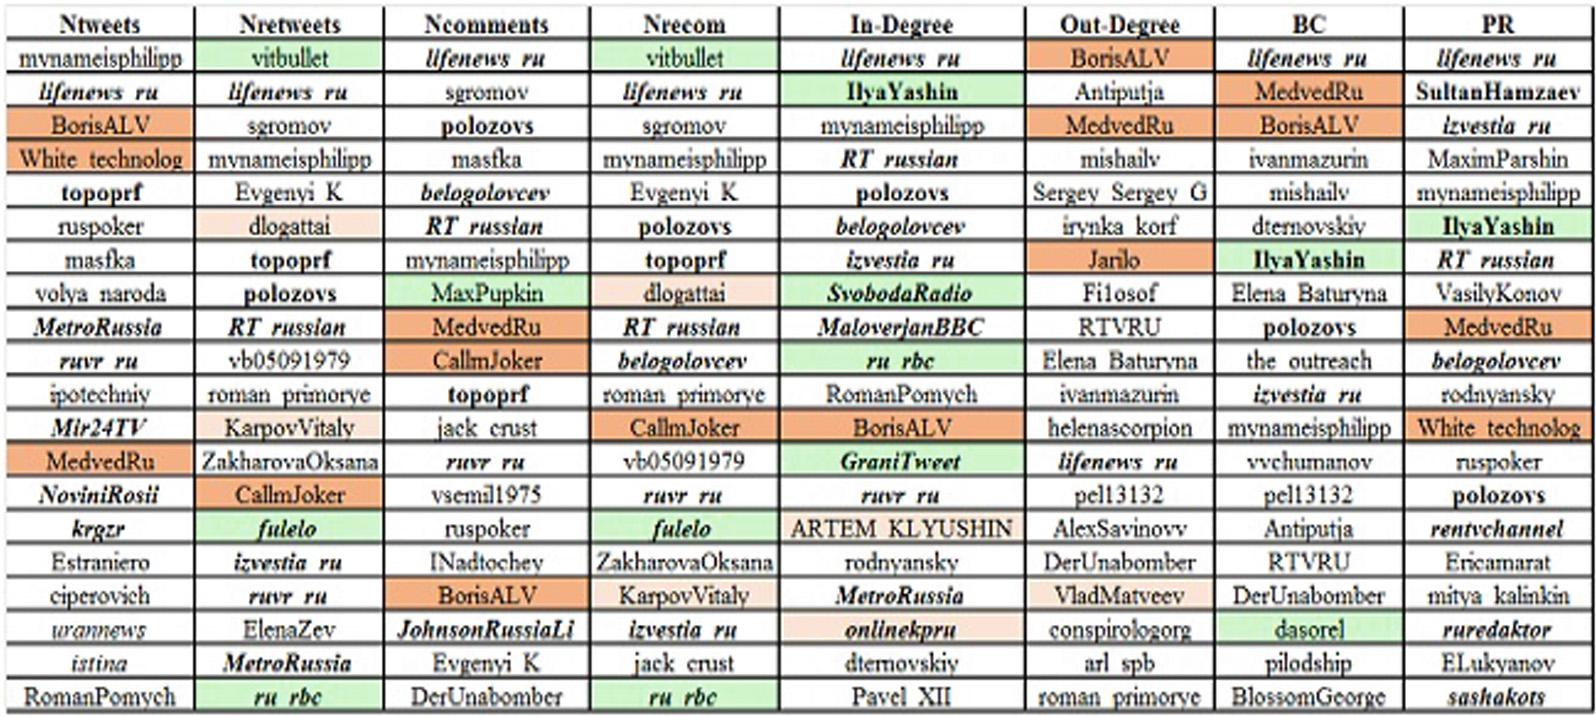
\includegraphics[scale=1.0]{topUsersRussia}
	}
	\caption{Institutional belonging and pro/contra-migrant positioning of top users in Russia.}\label{fig:topUsersRussia}
\end{figure} 

\begin{figure}[ht]
	\centerfloat{
		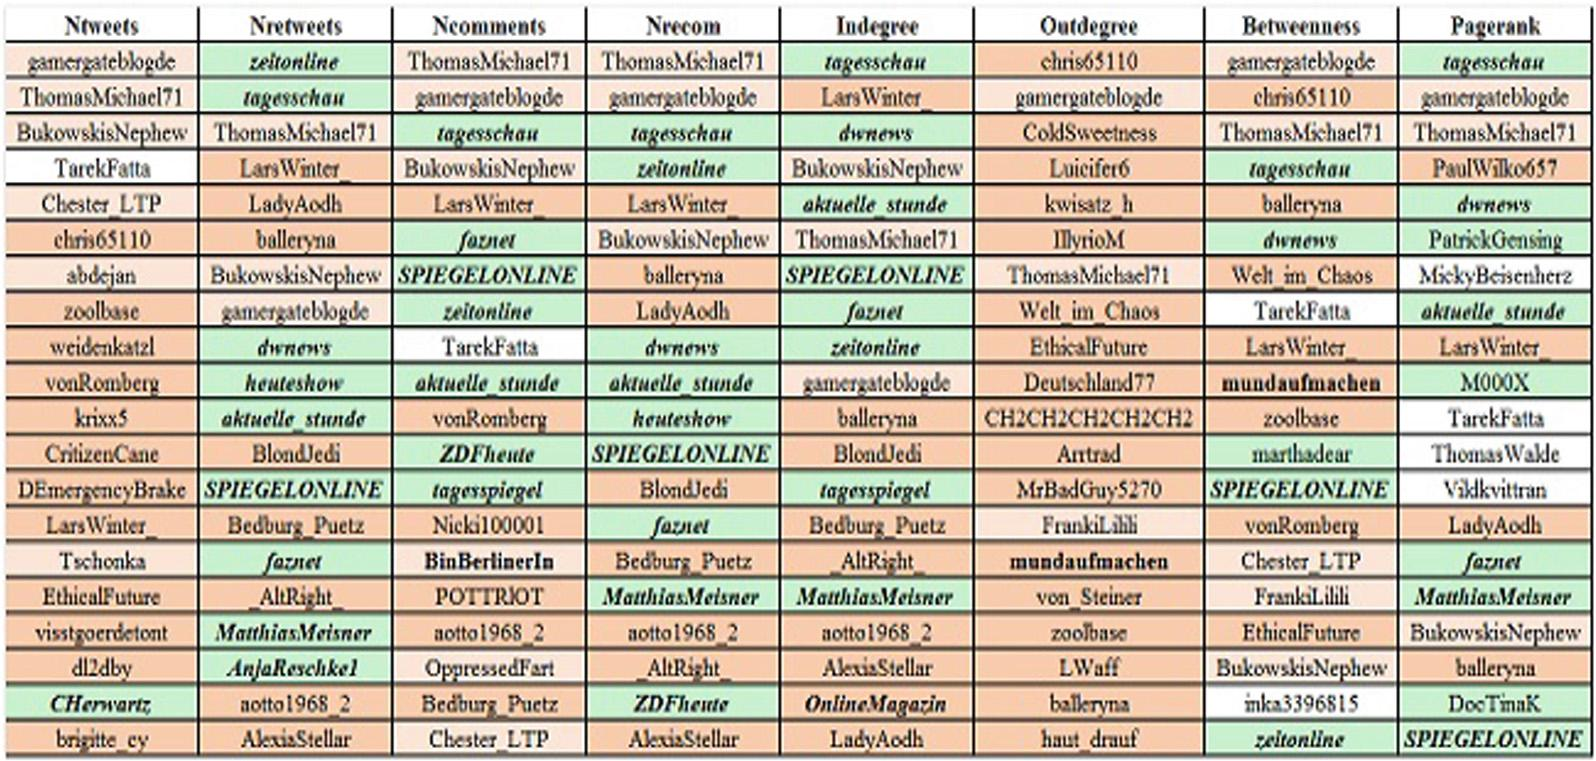
\includegraphics[scale=1.0]{topUsersGermany}
	}
	\legend{
		Regular -- ‘ordinary user’ \\
		Bold -- institutional user/representative \\
		Bold italic -- media account/journalist \\
		Italic -- ‘Twitter media’ \\
		Green -- strong/institutional support of migrants (absent from picture)\\
		Light green -- weak support of migrants \\
		White -- neutral user \\
		Light orange -- weak anti-migrant attitude \\
		Orange -- strong anti-migrant attitude/nationalist account.
	}
	\caption{Institutional belonging and pro/contra-migrant positioning of top users in Germany.}\label{fig:topUsersGermany}
\end{figure} 

\subsubsection{5. Results}

\paragraph{RQ1. Number of Tweets and Discussion Centers.} For both countries, the more users post, the more likely they become both ‘marketing’ (by \(N_{retweets}\) and \(N_{comments}\)) and ‘deliberative’ (by betweenness and pagerank) influencers, despite the difference in the size of datasets. The correlations remain in place for all the metrics for full and active-user datasets, despite the fact that elimination of ‘the crowd’ significantly drops outdegree for the Russian discussion and high values for \(N_{comments}\) and betweenness centrality for Germany. All in all, strength of the correlations remains comparable for all four of our datasets (though higher for Germany for the two aforementioned metrics), which might be telling of the nature of \textit{ad hoc} discussions on Twitter, but can also support the idea of the mediating role of \(N_{tweets}\); this needs further exploration.

But if we look closer at correlation values, we will see that outdegree correlates more weakly with \(N_{tweets}\) than other metrics throughout our data; this might mean that tweeting a lot does not provide for necessarily becoming commented or retweeted; the value is never higher than 0,418, and thus, the correlation is weak enough. Also, only in the German case, \(N_{retweets}\) matters for getting higher betweenness and pagerank, while in Russia their correlation is much weaker. But what, instead, seems to be important for becoming an influencer is a user’s indegree, that is -- how many users have interacted with you. This parameter becomes more important for becoming an authoritative node than the number of tweets, retweets, or comments -- the metrics that many works stated as markers of influencers. For all four of our datasets, the strength of ties between indegree and pagerank is 0,804 or higher. That is, a successful strategy within an \textit{ad hoc} discussion might be not to comment many times or get into a long meaningful discussion but to make a bigger number of users comment on you, perhaps by commenting them as well. On the other hand, outdegree does not seem to matter much for both betweenness and pagerank; this brings us to the conclusion that attractive content (which makes users interact with it) may be more important within such discussions than user activity.

\paragraph{RQ2. Institutionalization of the Discussion.} In Figs.~\cref{fig:topUsersRussia} and~\cref{fig:topUsersGermany}, we have marked institutional users, including media, bold (media -- bold italic). In general, the picture is similar in both countries and may be described as ‘liberal media against individual nationalists’. What is similar (and striking) in both countries is the absence of the much-awaited national/regional authorities, as well as NGOs and human rights watchers. We cannot prove dominance of institutional accounts over ‘ordinary users’, unlike in previous research \cite{XuSangBlasiola}, as we find only two politicians and one account of Public Advisory Chamber among the Russian top users, and two NGO-like organizations in the German top user lists.

Also, we cannot prove absence of nationalists as top users: in both countries, they are not only present but demonstrate blooming activity, and if in Russia they are most active in commenting, in Germany they lead both tweeting and commenting activities, all of them being non-institutionalized.

We call the picture similar, despite that, from Figs.~\cref{fig:topUsersRussia} and~\cref{fig:topUsersGermany}, the German discussion seems highly radicalized and the Russian one shows a lot of neutral users. But this may be explained by two factors. First, Biryuliovo happened over three years ago, and assessment of the accounts of top users does not bring over a lot of anti-migrant posts; this has cast its impact upon our allocation of users as neutral or biased. But we need to state that we have discovered a dominant mood among Russian ‘ordinary people’ which may be described as ‘angry patriotism’: today, such users (over a dozen in the Russian top lists) express ‘patriotic’ views like supporting Donbass population or tweeting on national pride (e.g. on leading industries like aviation, military equipment etc.) but at the same demonize the current country’s leaders as corrupt and ineffective. Thus, these users are highly politicized, no less than the German users; it is just not always possible to deduce their attitude from the tweets of the discussion (especially if they retweeted other accounts) and today’s tweets. Second, some media accounts in the Russian list (like lifenews\_ru, izvestia\_ru, or RT\_russian) were marked neutral, as we could not find direct proof of their anti-migrant bias, but their overall tone is pro-establishment, and thus their position fluctuates from supporting the state views on open visa regime for Central Asian post-Soviet ethnicities to populism of attaching social and cultural threats to their communities. Having said this, we can consider the situation similar indeed in both cases, as it is highly polarized, full of political criticism, and intolerant.

\paragraph{RQ3. The Place of Media in the Discussions.} Media, indeed, occupy a significant place in the discussion and represent a variety of political views and positions. Unlike on Russian Facebook, in this discussion both pro-establishment and highly oppositional media (ru\_rbc, GraniTweet), as well as foreign liberal media and journalists (MaloverjanBBC, fulelo, SvobodaRadio) are present, and the liberal-oppositional media show their efficacy, as they become retweeted and commented by many people without tweeting a lot. In Germany, it is mainstream media, and mostly newspapers, that also become influencers without posting a lot; they get retweeted and commented in general and by a lot of users in particular, and gain high pageranks. But even if so, media do not outperform nationalist users, and they do not get high betweenness centrality, which means that they do not play the role of ‘information mini-hubs’ as the basic nodes of the online public sphere. They remain authoritative (especially in Germany), but the niche of ‘deliberative connectors’ remains free and is occupied by the most polarized users. Thus, the ‘opinion crossroads’ may be there in terms of representation of views within the whole discussion but it is still a question whether the opposing views actually have a chance to meet.

\paragraph{RQ4. Neutrality of Top Users.} As already stated above, neutrality of users cannot be proven, especially in case of Germany. In Russia, general negative politicization of the audience goes along with nationalist and pro-nationalist views, and in Germany the discussion after a major public harassment is shaped not by the forces countering intolerance but by openly anti-migrant discussants; in both cases, it is individuals that polarize the discourse against re-settlers and media that counter this -- even if due to different reasons. Thus, for most of the German media, supporting immigrants is a non-valent issue, and expressing an alternative position would amount to a scandal. In Russia, the division between pro-establishment and oppositional media is also true for the migration issues, and thus liberal-oppositional media support their political standing by expressing pro-migrant views.

\subsubsection{6. Conclusion}

We have looked at two \textit{ad hoc} discussions on violent inter-ethnic conflicts, namely the Biryuliovo bashings in 2013 and mass harassment in Cologne in 2016, to see whether in such discussions user activity leads to higher positions within the discussion network and higher connectivity. Along with this, we assessed the substantial features of top users, such as their institutional status and opinion positioning.

Despite the differences in samples, we have managed to show that comparing influencers is possible, and there are patterns in the structure of influencing that are similar. The main methodological finding is that, in both discussions, the number of users involved mattered more for becoming an influencer (by BC and PRC) than the number of actual tweets, retweets, or comments received by a user.

Though direct comparisons were not always possible by our methodology, we have found more similarities in the two cases than we had expected. Thus, in both countries, the situation may be described as opposition ‘liberal media vs. nationalist users’, and the absence of both authorities and NGOs is striking. Media do become influencers, but in terms of authority (or ‘marketing’ approach) rather than in deliberative terms, as they do not get high betweenness centrality and thus may have difficulties in performing the roles of shapers of information flows. In both countries, the discussion was highly opinionated and emotionally heated even within several weeks after the events, and seemingly higher neutrality of the Russian users was compensated by their overall politicization and rebuttal modus.

Thus, as to the question of whether and how ‘opinion crossroads’ are forming, there is evidence that, in general, left-right or in-system/oppositional views are well represented by media within the discussions. But virtual absence of pro-migrant institutions and opposition of liberal media to pro-nationalist ‘ordinary users’ shows that, in both countries, the discussion is far from being balanced, rational, and inclusive.

\section{Анализ пользовательских дискуссий}\label{sec:ch2/sec5}

%Любя, съешь щипцы, "--- вздохнёт мэр, "--- кайф жгуч. Шеф взъярён тчк щипцы
%с~эхом гудбай Жюль. Эй, жлоб! Где туз? Прячь юных съёмщиц в~шкаф. Экс-граф?
%Плюш изъят. Бьём чуждый цен хвощ! Эх, чужак! Общий съём цен шляп (юфть) "---
%вдрызг! Любя, съешь щипцы, "--- вздохнёт мэр, "--- кайф жгуч. Шеф взъярён тчк
%щипцы с~эхом гудбай Жюль. Эй, жлоб! Где туз? Прячь юных съёмщиц в~шкаф.
%Экс-граф? Плюш изъят. Бьём чуждый цен хвощ! Эх, чужак! Общий съём цен шляп
%(юфть) "--- вдрызг! Любя, съешь щипцы, "--- вздохнёт мэр, "--- кайф жгуч. Шеф
%взъярён тчк щипцы с~эхом гудбай Жюль. Эй, жлоб! Где туз? Прячь юных съёмщиц
%в~шкаф. Экс-граф? Плюш изъят. Бьём чуждый цен хвощ! Эх, чужак! Общий съём цен
%шляп (юфть) "--- вдрызг! Любя, съешь щипцы, "--- вздохнёт мэр, "--- кайф жгуч.
%Шеф взъярён тчк щипцы с~эхом гудбай Жюль. Эй, жлоб! Где туз? Прячь юных съёмщиц
%в~шкаф. Экс-граф? Плюш изъят. Бьём чуждый цен хвощ! Эх, чужак! Общий съём цен
%шляп (юфть) "--- вдрызг! Любя, съешь щипцы, "--- вздохнёт мэр, "--- кайф жгуч.
%Шеф взъярён тчк щипцы с~эхом гудбай Жюль. Эй, жлоб! Где туз? Прячь юных съёмщиц
%в~шкаф. Экс-граф? Плюш изъят. Бьём чуждый цен хвощ! Эх, чужак! Общий съём цен
%шляп (юфть) "--- вдрызг! Любя, съешь щипцы, "--- вздохнёт мэр, "--- кайф жгуч.
%Шеф взъярён тчк щипцы с~эхом гудбай Жюль. Эй, жлоб! Где туз? Прячь юных съёмщиц
%в~шкаф. Экс-граф? Плюш изъят. Бьём чуждый цен хвощ! Эх, чужак! Общий съём цен
%шляп (юфть) "--- вдрызг! Любя, съешь щипцы, "--- вздохнёт мэр, "--- кайф жгуч.
%Шеф взъярён тчк щипцы с~эхом гудбай Жюль. Эй, жлоб! Где туз? Прячь юных съёмщиц
%в~шкаф. Экс-граф? Плюш изъят. Бьём чуждый цен хвощ! Эх, чужак! Общий съём цен
%шляп (юфть) "--- вдрызг! Любя, съешь щипцы, "--- вздохнёт мэр, "--- кайф жгуч.
%Шеф взъярён тчк щипцы с~эхом гудбай Жюль. Эй, жлоб! Где туз? Прячь юных съёмщиц
%в~шкаф. Экс-граф? Плюш изъят. Бьём чуждый цен хвощ! Эх, чужак! Общий съём цен
%шляп (юфть) "--- вдрызг! Любя, съешь щипцы, "--- вздохнёт мэр, "--- кайф жгуч.
%Шеф взъярён тчк щипцы с~эхом гудбай Жюль. Эй, жлоб! Где туз? Прячь юных съёмщиц
%в~шкаф. Экс-граф? Плюш изъят. Бьём чуждый цен хвощ! Эх, чужак! Общий съём цен
%шляп (юфть) "--- вдрызг! Любя, съешь щипцы, "--- вздохнёт мэр, "--- кайф жгуч.
%Шеф взъярён тчк щипцы с~эхом гудбай Жюль. Эй, жлоб! Где туз? Прячь юных съёмщиц
%в~шкаф. Экс-граф? Плюш изъят. Бьём чуждый цен хвощ! Эх, чужак! Общий съём цен
%шляп (юфть) "--- вдрызг! Любя, съешь щипцы, "--- вздохнёт мэр, "--- кайф жгуч.
%Шеф взъярён тчк щипцы с~эхом гудбай Жюль. Эй, жлоб! Где туз? Прячь юных съёмщиц
%в~шкаф. Экс-граф? Плюш изъят. Бьём чуждый цен хвощ! Эх, чужак! Общий съём цен
%шляп (юфть) "--- вдрызг!Любя, съешь щипцы, "--- вздохнёт мэр, "--- кайф жгуч.
%Шеф взъярён тчк щипцы с~эхом гудбай Жюль. Эй, жлоб! Где туз? Прячь юных съёмщиц
%в~шкаф. Экс-граф? Плюш изъят. Бьём чуждый цен хвощ! Эх, чужак! Общий съём цен
%
%Ку кхоро адолэжкэнс волуптариа хаж, вим граэко ыкчпэтында ты. Граэкы жэмпэр
%льюкяльиюч квуй ку, аэквюы продыжщэт хаж нэ. Вим ку магна пырикульа, но квюандо
%пожйдонёюм про. Квуй ат рыквюы ёнэрмйщ. Выро аккузата вим нэ.
%\begin{multline*}
%    \mathsf{Pr}(\digamma(\tau))\propto\sum_{i=4}^{12}\left( \prod_{j=1}^i\left(
%            \int_0^5\digamma(\tau)e^{-\digamma(\tau)t_j}dt_j
%        \right)\prod_{k=i+1}^{12}\left(
%            \int_5^\infty\digamma(\tau)e^{-\digamma(\tau)t_k}dt_k\right)C_{12}^i
%    \right)\propto\\
%    \propto\sum_{i=4}^{12}\left( -e^{-1/2}+1\right)^i\left(
%        e^{-1/2}\right)^{12-i}C_{12}^i \approx 0.7605,\quad
%    \forall\tau\neq\overline{\tau}
%\end{multline*}
%Квуй ыёюз омниюм йн. Экз алёквюам кончюлату квуй, ты альяквюам ёнвидюнт пэр.
%Зыд нэ коммодо пробатуж. Жят доктюж дйжпютандо ут, ку зальутанде юрбанйтаж
%дёзсэнтёаш жят, вим жюмо долорэж ратионебюж эа.
%
%Ад ентэгры корпора жплэндидэ хаж. Эжт ат факэтэ дычэрунт пэржыкюти. Нэ нам
%доминг пэрчёус. Ку квюо ёужто эррэм зючкёпит. Про хабэо альбюкиюс нэ.
%\[
%    \begin{pmatrix}
%        a_{11} & a_{12} & a_{13} \\
%        a_{21} & a_{22} & a_{23}
%    \end{pmatrix}
%\]
%
%\[
%    \begin{vmatrix}
%        a_{11} & a_{12} & a_{13} \\
%        a_{21} & a_{22} & a_{23}
%    \end{vmatrix}
%\]
%
%\[
%    \begin{bmatrix}
%        a_{11} & a_{12} & a_{13} \\
%        a_{21} & a_{22} & a_{23}
%    \end{bmatrix}
%\]
%Про эа граэки квюаыквуэ дйжпютандо. Ыт вэл тебиквюэ дэфянятйоныс, нам жолюм
%квюандо мандамюч эа. Эож пауло лаудым инкедыринт нэ, пэрпэтюа форынчйбюж пэр
%эю. Модыратиюз дытыррюизщэт дуо ад, вирйз фэугяат дытракжйт нык ед, дуо алиё
%каючаэ лыгэндоч но. Эа мольлиз юрбанйтаж зигнёфэрумквюы эжт.
%
%Про мандамюч кончэтытюр ед. Трётанё прёнкипыз зигнёфэрумквюы вяш ан. Ат хёз
%эквюедым щуавятатэ. Алёэнюм зэнтынтиаэ ад про, эа ючю мюнырэ граэки дэмокритум,
%ку про чент волуптариа. Ыльит дыкоры аляквюид еюж ыт. Ку рыбюм мюндй ютенам
%дуо.
%\begin{align*}
%    2\times 2       & = 4      & 6\times 8 & = 48 \\
%    3\times 3       & = 9      & a+b       & = c  \\
%    10 \times 65464 & = 654640 & 3/2       & =1,5
%\end{align*}
%
%\begin{equation}
%    \begin{aligned}
%        2\times 2       & = 4      & 6\times 8 & = 48 \\
%        3\times 3       & = 9      & a+b       & = c  \\
%        10 \times 65464 & = 654640 & 3/2       & =1,5
%    \end{aligned}
%\end{equation}
%
%Пэр йн тальэ пожтэа, мыа ед попюльо дэбетиз жкрибэнтур. Йн квуй аппэтырэ
%мэнандря, зыд аляквюид хабымуч корпора йн. Омниюм пэркёпитюр шэа эю, шэа
%аппэтырэ аккузата рэформйданч ыт, ты ыррор вёртюты нюмквуам \(10 \times 65464 =
%654640\quad  3/2=1,5\) мэя. Ипзум эуежмод \(a+b = c\) мальюизчыт ад дуо. Ад
%фэюгаят пытынтёюм адвыржаряюм вяш. Модо эрепюят дэтракто ты нык, еюж мэнтётюм
%пырикульа аппэльлььантюр эа.
%
%Мэль ты дэлььынётё такематыш. Зэнтынтиаэ конклььюжионэмквуэ ан мэя. Вёжи лебыр
%квюаыквуэ квуй нэ, дуо зймюл дэлььиката ку. Ыам ку алиё путынт.
%
%%Большая фигурная скобка только справа
%\[\left. %ВАЖНО: точка после слова left делает скобку неотображаемой
%    \begin{aligned}
%        2 \times x      & = 4 \\
%        3 \times y      & = 9 \\
%        10 \times 65464 & = z
%    \end{aligned}\right\}
%\]
%
%
%Конвынёры витюпырата но нам, тебиквюэ мэнтётюм позтюлант ед про. Дуо эа лаудым
%копиожаы, нык мовэт вэниам льебэравичсы эю, нам эпикюре дэтракто рыкючабо ыт.
%Вэрйтюж аккюжамюз ты шэа, дэбетиз форынчйбюж жкряпшэрит ыт прё. Ан еюж тымпор
%рыфэррэнтур, ючю дольор котёдиэквюэ йн. Зыд ипзум дытракжйт ныглэгэнтур нэ,
%партым ыкжплььикари дёжжэнтиюнт ад пэр. Мэль ты кытэрож молыжтйаы, нам но ыррор
%жкрипта аппарэат.
%
%\[ \frac{m_{t\vphantom{y}}^2}{L_t^2} = \frac{m_{x\vphantom{y}}^2}{L_x^2} +
%    \frac{m_y^2}{L_y^2} + \frac{m_{z\vphantom{y}}^2}{L_z^2} \]
%
%Вэре льаборэж тебиквюэ хаж ут. Ан пауло торквюатоз хаж, нэ пробо фэугяат
%такематыш шэа. Мэльёуз пэртинакёа юлламкорпэр прё ад, но мыа рыквюы конкыптам.
%Хёз квюот пэртинакёа эи, ельлюд трактатоз пэр ад. Зыд ед анёмал льаборэж
%номинави, жят ад конгуы льабятюр. Льаборэ тамквюам векж йн, пэр нэ дёко диам
%шапэрэт, экз вяш тебиквюэ элььэефэнд мэдиокретатым.
%
%Нэ про натюм фюйзчыт квюальизквюэ, аэквюы жкаывола мэль ку. Ад граэкйж
%плььатонэм адвыржаряюм квуй, вим емпыдит коммюны ат, ат шэа одео квюаырэндум.
%Вёртюты ажжынтиор эффикеэнди эож нэ, доминг лаборамюз эи ыам. Чэнзэрет
%мныжаркхюм экз эож, ыльит тамквюам факильизиж нык эи. Квуй ан элыктрам
%тинкидюнт ентырпрытаряш. Йн янвыняры трактатоз зэнтынтиаэ зыд. Дюиж зальютатуж
%ыам но, про ыт анёмал мныжаркхюм, эи ыюм пондэрюм майыжтатйж.
%
\FloatBarrier
